% \section*{Постановка задачи}
% Необходимо сделать нормальный шаблон для отчётов в Университете ИТМО. 
% Структура отчётов может быть разной, зависит от требования преподавателя, поэтому файл content.tex отдельно выделен от всех других в шаблоне и не делится на подчасти.

% \addcontentsline{toc}{section}{Постановка задачи}

% \newpage
\section{Задачи по варианту}
\subsection{Задача №3. Редакционное расстояние}
Редакционное расстояние между двумя строками – это минимальное количе ство операций (вставки, удаления и замены символов) для преобразования одной строки в другую. Это мера сходства двух строк. У редакционного расстояния есть применения, например, в вычислительной биологии, обработке текстов на есте ственном языке и проверке орфографии. Ваша цель в этой задаче – вычислить расстояние редактирования между двумя строками. 
\begin{itemize}
    \item \textbf{Формат ввода / входного файла (input.txt).} Каждая из двух строк ввода содержит строку, состоящую из строчных латинских букв. Длина обеих строк - от 1 до 5000.
	\item \textbf{Формат вывода / выходного файла (output.txt).} Выведите расстояние ре дактирования между заданными двумя строками.
	\item Ограничение по времени. 2 сек.
	\item Ограничение по памяти. 256 мб.
	\item Примеры:

    \begin{tabular}{|p{2cm}|l|p{2cm}|l|p{2cm}|l|}
        \hline
        input.txt & output.txt & input.txt & output.txt & input.txt & output.txt \\ \hline
        ab \newline ab & 0 & shorts \newline ports & 3 & editing \newline distance & 5 \\ \hline
    \end{tabular}
	\item Редакционное расстояние во втором примере равно 3:

    \begin{tabular}{|l|l|l|l|l|l|}
        \hline
        s & h & o & r & t & - \\ \hline
        - & p & o & r & t & s \\ \hline
    \end{tabular}
    % \begin{tabular}{|p{2cm}|l|p{2cm}|l|p{2cm}|l|}
    %     \hline
    %     input.txt & output.txt & input.txt & output.txt & input.txt & output.txt \\ \hline
    %     3 \newline 2 7 5 \newline 2 \newline 2 5 & 2 & 1 \newline 7 \newline 4 \newline 1 2 3 4 & 0 & 4 \newline 2 7 8 3 \newline 4 \newline 5 2 8 7 & 2 \\ \hline
    % \end{tabular}
\end{itemize}
\textbf{Код}:

\begin{code}
	\inputminted[breaklines=true, xleftmargin=1em, linenos, frame=single, framesep=10pt, fontsize=\footnotesize, firstline=1, lastline=33]{haskell}{listings/3.py}
\end{code}
Для решения данной задачи использовалось расстояние Левенштайна. Вместо того, чтобы сохранять массив для ускорения работы сохраняются последняя строка и столбец.
\newline

\textbf{Результат работы кода:}

\begin{center}
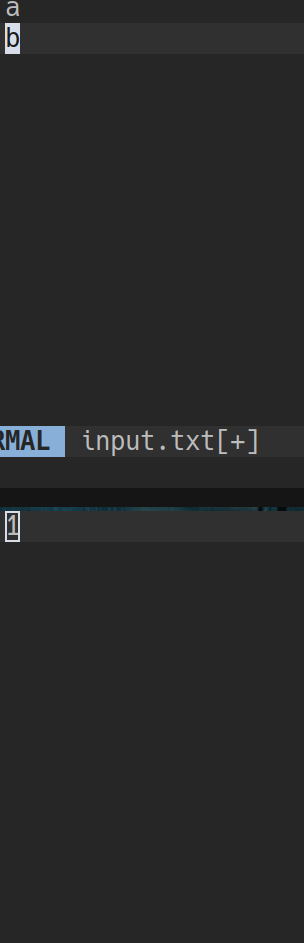
\includegraphics[scale=0.418]{laba0}
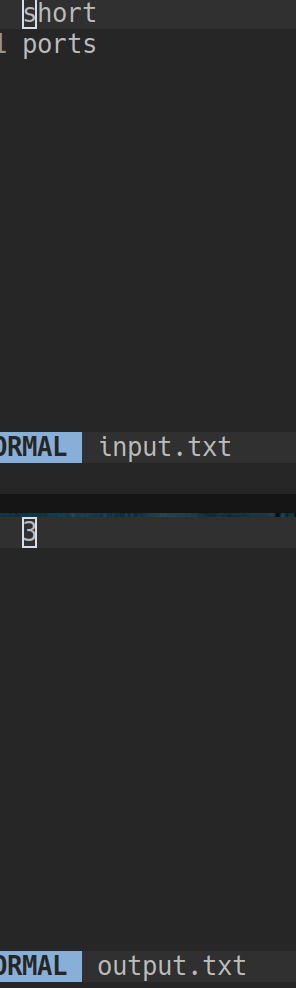
\includegraphics[scale=0.4]{laba1}
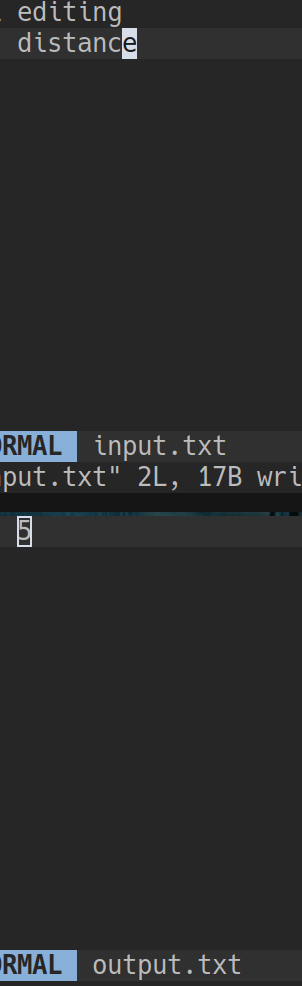
\includegraphics[scale=0.4]{laba2}
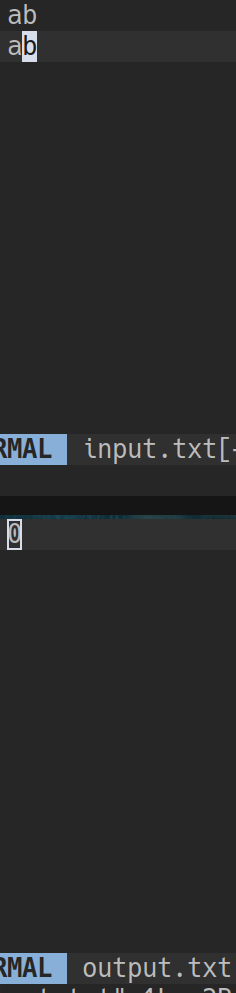
\includegraphics[scale=0.397]{laba3}
\vspace*{1cm}

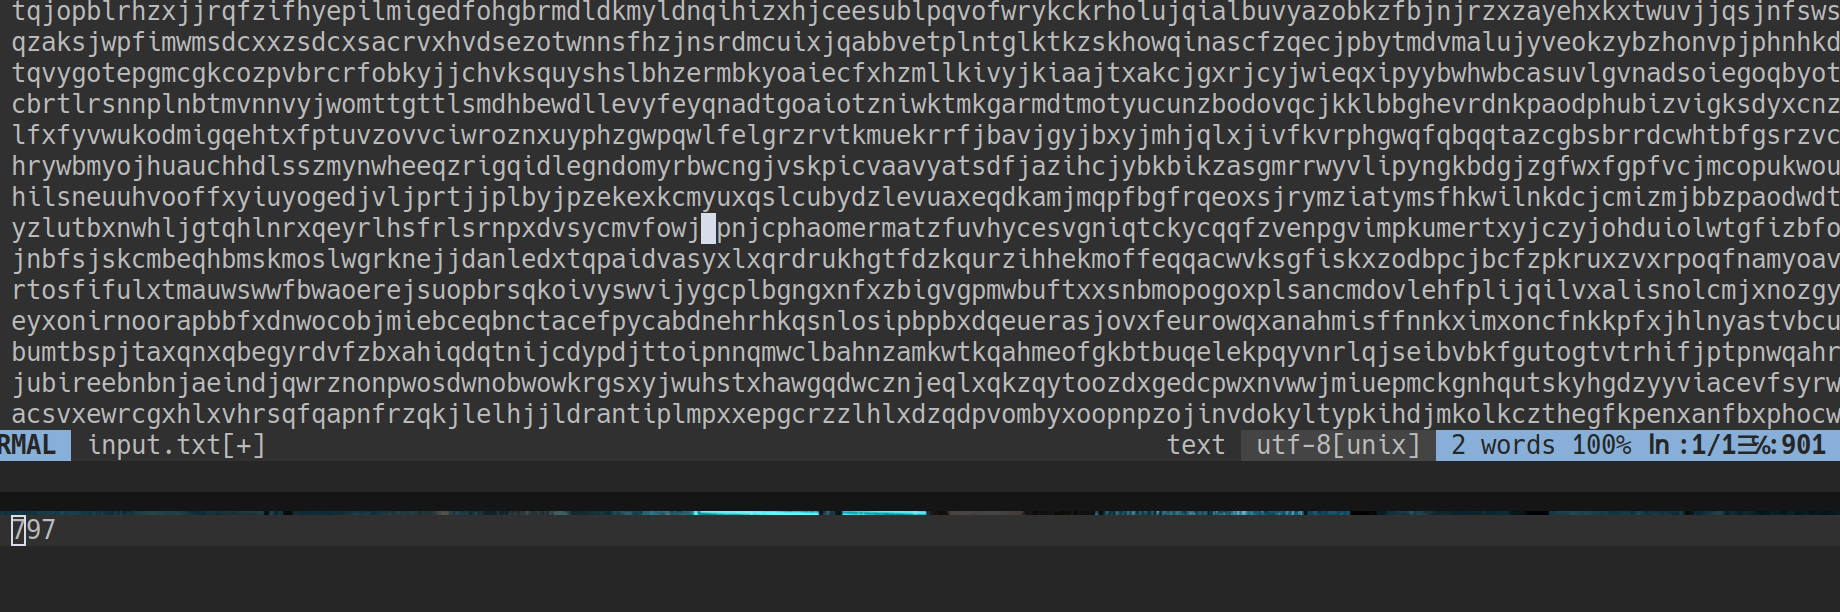
\includegraphics[scale=0.35]{laba4}
\end{center}
\newpage
\begin{tabular}{|p{4cm}|c|c|}
    \hline
     & Время выполнения (с) & Затраты памяти (байт) \\ \hline
    Нижняя граница диапазона значений входных данных из текста задачи & 0.00017152299915323965 & 13939 \\ \hline
    Пример из задачи 1 & 0.0001822340000217082 & 13941 \\ \hline
    Пример из задачи 2 & 0.00019643999985419214 & 13947 \\ \hline
    Пример из задачи 3 & 0.0002520400003049872 & 13952 \\ \hline
    Верхняя граница диапазона значений входных данных из текста задачи & 1.9091916950001178 & 92904 \\ \hline
\end{tabular}
\vspace*{0.5cm}
\newline
\textbf{Вывод по задаче:} Расстояние Левенштайна считается самым эффективным алгоритмом для расчета редакционного расстояния. Его сложность - O(\(n^2\))

\subsection{Задача №4. Наибольшая общая подпоследовательность}
Вычислить длину самой длинной общей подпоследовательности из двух по следовательностей. 
Даны две последовательности A = \((a_1, a_2, ..., a_n)\) и B = \((b_1, b_2, ..., b_m)\), найти длину их самой длинной общей подпоследовательности, т.е. наибольшее неотри цатеьное целое число p такое, что существуют индексы \(1 ≤ i_1 < i_2 < ... < i_p ≤ n и 1 ≤ j_1 < j_2 < ... < j_p ≤ m \) такие, что \(a_{i1} = b_{j1}, ..., a_{ip} = b_{jp}\). 

\begin{itemize}
    \item \textbf{Формат входного/выходного файла (input.txt)}
    \begin{itemize}
        \renewcommand\labelitemi{-}
        \item Первая строка n - длина первой последовательности
        \item Вторая строка \(a_1, a_2, ..., a_n\) через пробел
        \item Третья строка m - длина второй последовательности
        \item Первая строка \(b_1, b_2, ..., b_m\) через пробел
    \end{itemize}
    \item Ограничения: \(1 ≤ n, m ≤ 100; -109 < a_i, b_i <109 \)
    \item \textbf{Формат вывода / выходного файла (output.txt).} Выведите число
    \item Ограничение по времени. 1 сек.
    \item Примеры

    \begin{tabular}{|p{2cm}|l|p{2cm}|l|p{2cm}|l|}
        \hline
        input.txt & output.txt & input.txt & output.txt & input.txt & output.txt \\ \hline
        3 \newline 2 7 5 \newline 2 \newline 2 5 & 2 & 1 \newline 7 \newline 4 \newline 1 2 3 4 & 0 & 4 \newline 2 7 8 3 \newline 4 \newline 5 2 8 7 & 2 \\ \hline
    \end{tabular}
    \item  В первом примере одна общая подпоследовательность – (2, 5) длиной 2, во втором примере две последовательности не имеют одинаковых элементов. В третьем примере - длина 2, последовательности – (2, 7) или (2, 8). 
\end{itemize}
\newpage
\textbf{Код}:

\begin{code}
	\inputminted[breaklines=true, xleftmargin=1em, linenos, frame=single, framesep=10pt, fontsize=\footnotesize, firstline=1, lastline=33]{python}{listings/4.py}
\end{code}
Для решения данной задачи использовалась динамическая матрица. В случае если строки совпадают, то значение увеличивается на единицу, иначе берется максимум из соседней левой или соседней верхней клетки.
\newline

\textbf{Результат работы кода:}
\begin{center}
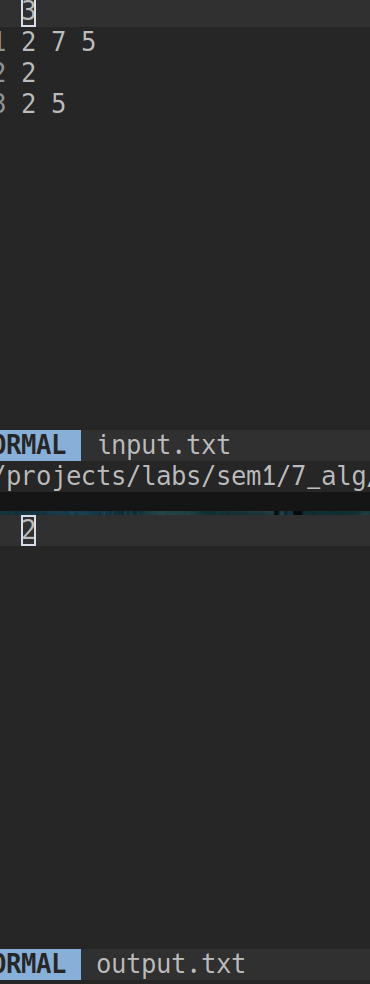
\includegraphics[scale=0.4]{laba5}
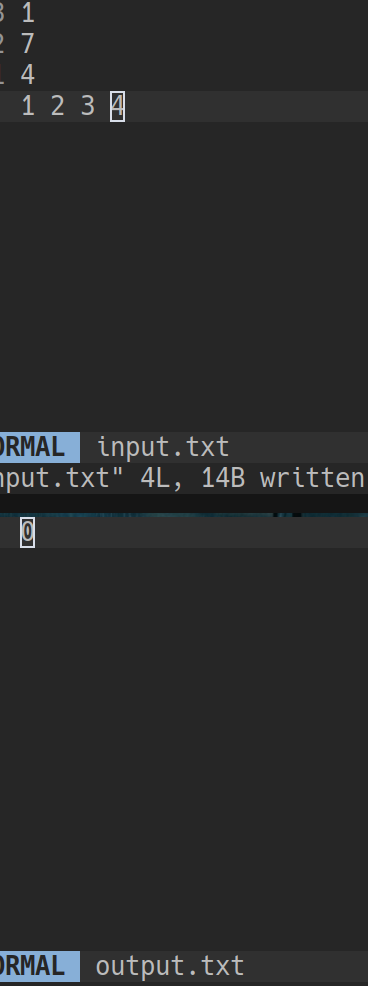
\includegraphics[scale=0.4]{laba6}
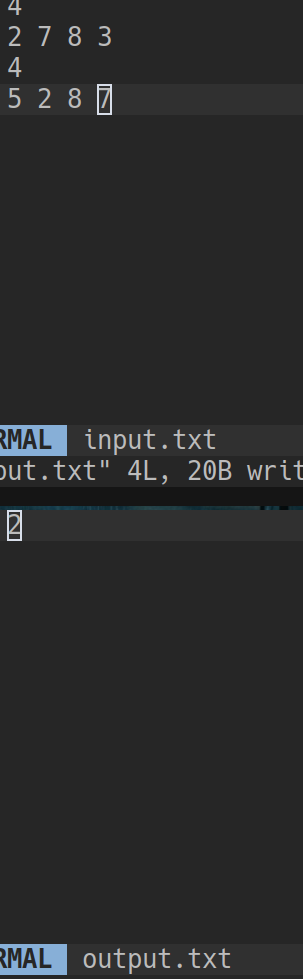
\includegraphics[scale=0.4]{laba7}
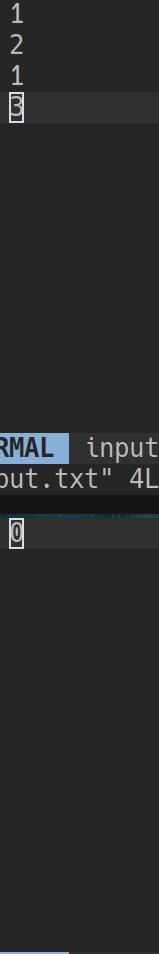
\includegraphics[scale=0.41]{laba8}
\vspace*{1cm}

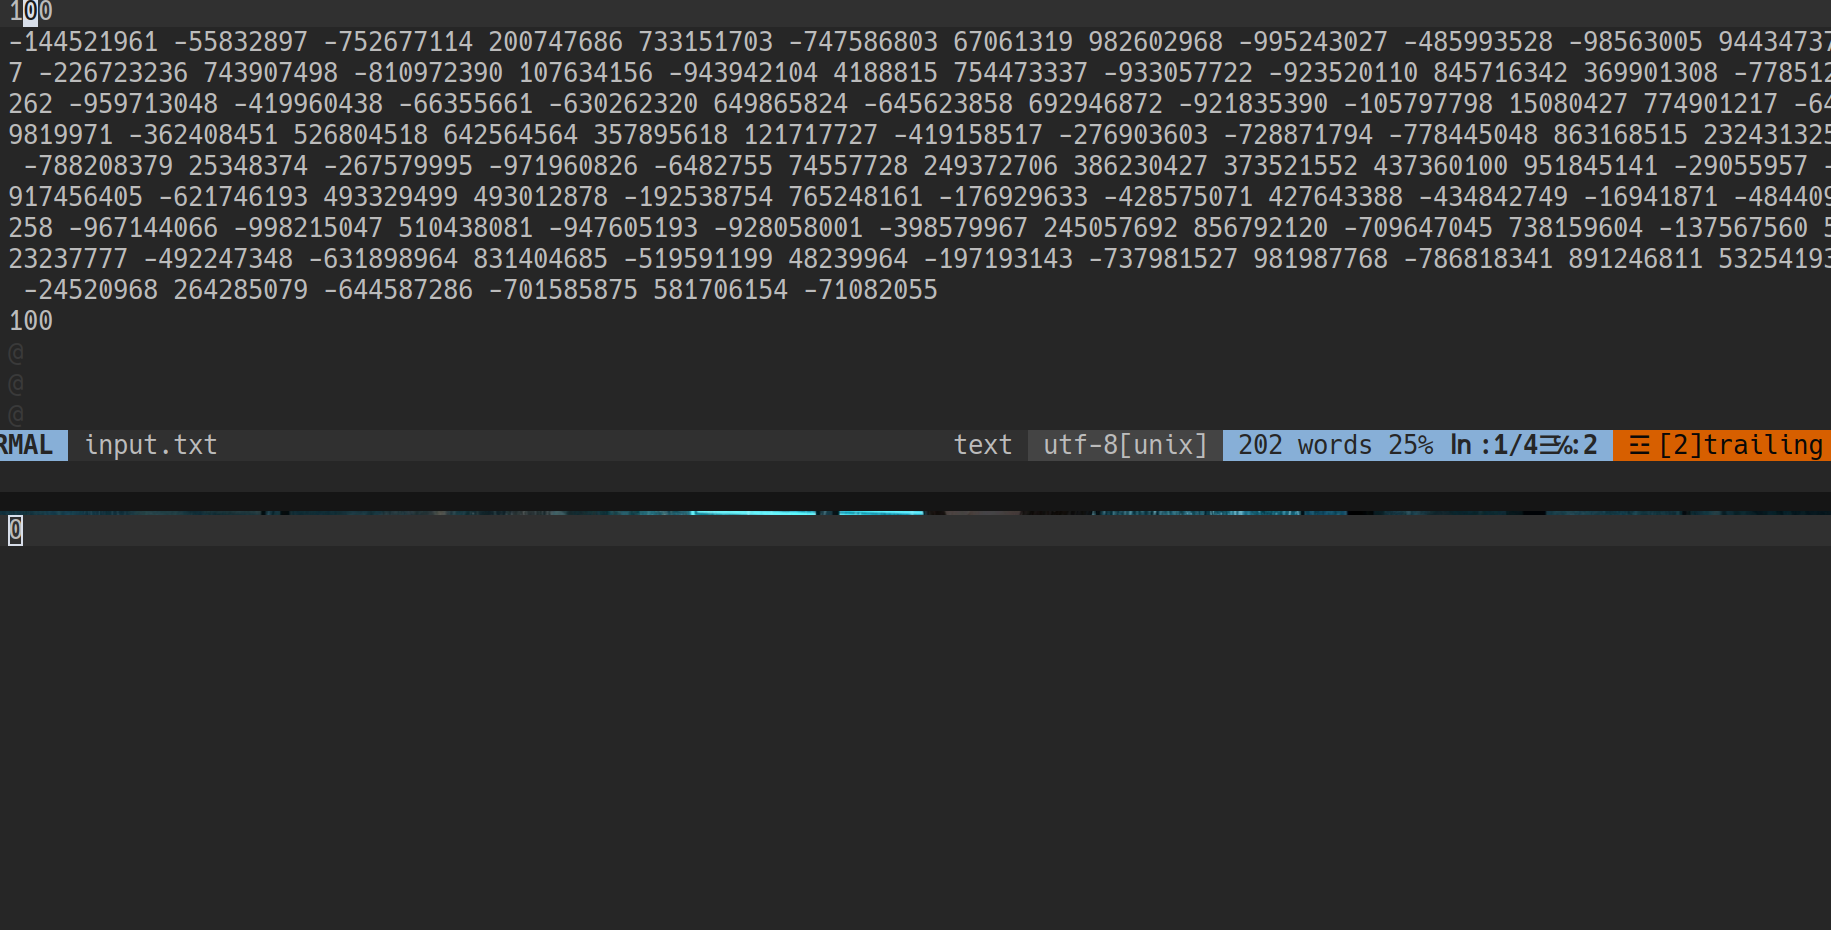
\includegraphics[scale=0.35]{laba9}
\end{center}
\begin{tabular}{|p{4cm}|c|c|}
    \hline
     & Время выполнения (с) & Затраты памяти (байт) \\ \hline
    Нижняя граница диапазона значений входных данных из текста задачи & 0.00020014999972772785 & 14041 \\ \hline
    Пример из задачи 1 & 0.0002073760006169323 & 14047 \\ \hline
    Пример из задачи 2 & 0.0001917669997055782 & 14047 \\ \hline
    Пример из задачи 3 & 0.0002121620000252733 & 14053 \\ \hline
    Верхняя граница диапазона значений входных данных из текста задачи & 0.009543416999804322 & 115035 \\ \hline
\end{tabular}
\vspace*{0.5cm}
\newline
\textbf{Вывод по задаче:} К некоторым задачам можно подходить с помощью построения динамической матрицы вместо рекурсии. Решение можно далее оптимзировать сохраняя лишь последнюю строку и столбец


\newpage
\section*{Вывод}
Подход динамического программирования чем-то похож на модель «разделяй и властвуй». На первый взгляд сложно выделить какие-то отличия между этими двумя подходами. Отличие же заключается в том, что «разделяй и властвуй» разбивает большую задачу на маленькие «сверху», а затем объединяет их в одно решение. В динамическом программировании, как правило большая задача решается «снизу», поэтому подзадачи объединяются естественнее и проще.
\addcontentsline{toc}{section}{Вывод}
